\subsection{Overview}
Quantum information theory provides a framework to quantify the power of quantum theory compared to classical communication theory. Over the last decades, the field has flourished compelled to set realistic boundaries to the promises of quantum advantages in fields like quantum communication and computing. An important feature of quantum theory lies in the statistical correlations produced by local measurements of a quantum system. The simplest example of quantum correlations are the ones produced by projective measurements on a maximally-entangled state of two qubits, also known as a Bell pair state. Such correlations are the basic resource of bipartite quantum information theory, where various equivalences are known: one shared Bell pair plus two bits of classical information can be used to teleport one  qubit and, conversely, one shared Bell pair state plus a single qubit can be used to send two bits of classical information via superdense coding. Exploring the fundamental limits of quantum over classical advantages in these scenarios is crucial, and it will be the primary objective of this work.
\par
In the early years of the current century, Ben Toner and David Bacon developed a protocol which proves that any prediction based on projective measurements on an entangled Bell pair state could be simulated by communicating only two classical bits \cite{toner2003}. Very recently, Martin Renner, Armin Tavakoli and Marco Tulio Quintino, have extended such result to a most generalised set of measurements, the positive operator-valued measures \cite{renner2022}.
Following up such generalisation, we will show by classical and quantum computer-based experiments that a qubit transmission can be simulated classically with a total cost of two bits for any general measurement, either in a prepare-and-measure or an entanglement scenario. 
\par
Before starting to describe the different computational experiments we have carried out to achieve such goal, it is worth spending next sections to introduce some preliminary concepts and notations that have been used extensively throughout this work, specifically the definition of positive operator-valued measures, the set-up of both the prepare-and-measure and Bell scenarios and the particular details of the classical simulation protocols applied to such scenarios.
\par
\subsection{Positive operator-valued measures}\label{section:povms}
Even when most of the introductory textbooks on quantum mechanics describe the measurement postulates using projective measurements only, there exists a more general and less restrictive set of measurements called Positive Operator-Valued Measures or POVMs, see \cite{nielsen2000}\cite{peres1995}. The underlying formalism behind POVMs is uniquely well adapted for some applications where the main focus is on describing the probabilities of the different measurement outcomes rather than on the post-measurement state of the system. This is of particular interest in quantum communication and quantum information, where a more comprehensive formalism for the description of the measurements is needed, and highlights how important are the results from \cite{renner2022}, where all the results are extended to POVMs without any loss of generalisation regarding the the classical simulation cost of the protocol. For reference, we define explicitely a POVM as a set $\mathbb P=\{B_b\}$ with $b=1,...,N$ positive semidefinite operators acting on a Hilbert space $\mathcal{H}^{d_Q}$ of dimension $d_{Q}$, which satisfies the closure property $\sum_{b=1}^{N} B_{b} = \mathbb{1}$. The operator $B_{b}$ is called a POVM element, and it is associated to the outcome $b$ of the POVM. In this work we will use extensively the property which states that every qubit POVM can be written as a coarse graining of rank-1 projectors \cite{barrett2002}, such that we will restrict our POVM calculations to the case of rank-1 projectors.

\subsection{Prepare-and-measure scenario}\label{section:pm}
As for many other communication protocols we have two well-known characters playing different roles in the quantum prepare-and-measure set-up: Alice and Bob. Such scenario starts with Alice preparing a random quantum state and sending it to Bob. In a general set-up, i.e. not restricted to single qubit communication, the state prepared by Alice is a state of dimension $d_Q$ described by a positive semidefinite density matrix $\rho \in \mathcal{L}( \mathbb{C}_{d_Q}), \rho \ge 0$ with unit trace $tr(\rho)=1$. Once the state is prepared and communicated by Alice, Bob then receives it and performs a random quantum measurement on it, obtaining an outcome $b$. In the case of general POVM measurements $\mathbb P=\{B_b\}$ as described in section \ref{section:povms}, the probability of outcome $b$ when performing the measurement on the state $\rho$ is given by Born's rule,

\begin{equation}\label{eq:prob_quantum}
p_Q(b|\rho,\{B_b\}) = tr(\rho B_b)
\end{equation}

In the context of this work, we are interested in the classical counterpart of the quantum prepare-and-measure scenario, where the probability distributions predicted by the quantum theory (\ref{eq:prob_quantum}) are reproduced classically. All these classical counterparts of existing quantum protocols, see examples in \cite{cerf2000}, \cite{toner2003} and \cite{renner2022}, require a shared randomness $\lambda$ among Alice and Bob subject to some probability function $\pi(\lambda)$ to correlate their classical communication strategies. As it is not possible to reproduce these correlations without communication, a classical message $c$ which encodes classically the quantum state $\rho$ taking its value from a $d_C$-valued alphabet $\{1,...,d_C\}$ is also required. Alice's actions are therefore described by the conditional probability $p_A(c|\rho,\lambda)$, whereas Bob's actions are similarly described by the conditional probability $p_B(b|\{B_b\},c,\lambda)$. If we consider both probabilities, the correlations from the classical counterpart become

\begin{equation}\label{eq:prob_classic}
p_C(b|\rho,\{B_b\}) = \int_{\lambda} d\lambda\ \pi(\lambda) \sum_{c=1}^{d_C} p_A(c|\rho, \lambda) p_B(b|\{B_b\}, c, \lambda)
\end{equation}

Given equations (\ref{eq:prob_quantum}) and (\ref{eq:prob_classic}), the classical simulation would be considered successful when, for every random state and POVM, the classical probability distribution reproduces the quantum predictions, i.e.

\begin{equation}
\forall \rho, \{B_b\}:\quad p_C(b|\rho,\{B_b\}) = p_Q(b|\rho,\{B_b\})
\end{equation}

\subsection{Bell scenario}
In a Bell scenario, there is a bipartite quantum system of two entangled and separated qudits, one with Alice and another one with Bob. 
Alice chooses a random local measurement, and produces an output according to the distribution of her measurement elements. Following the same procedure, Bob chooses his own random local measurement and produces an outcome. Even if both outcomes appear random, their joint probabilities are correlated. We refer to these correlations as Bell correlations.

Similarly to the prepare-and-measure case described in section \ref{section:pm}, it is not possible to reproduce the correlations using a classical protocol with shared random variables without allowing classical communication among Alice and Bob once they have selected their measurements \cite{bell1964}. The main question here is to determine how much classical communication is needed to reproduce the probability distributions.

As \cite{renner2022} shows, it is straight-forward to adapt the prepare-and-measure classical scenario to any entangled qudit-qubit state. Here Alice chooses a random local POVM on a $d_Q$-dimensional quantum system, and produces an output according to the marginal distribution of her POVM elements. Based on her output, she computes Bob's entangled qubit post-measurement state, which is sent to Bob using the prepare-and-measure scenario. Given that Bob's post-measurement qubit state is communicated by Alice using the existing prepare-and-measure classical protocol, the classical cost of the qubit transmission will be exactly the same. 

In addition to this, we will discuss in the next sections other Bell scenarios where the entangled state is a Bell singlet state and the classical simulation cost is reduced to one bit.


\subsection{Classical simulation protocols}
\subsubsection{Prepare-and-measure with one qubit}
\textit{$d_Q=2$}
\begin{equation}
tr(\rho B_b) = p_b(1 + \vec{x} \cdot \vec{y}_b) 
\end{equation}

\begin{equation}
B_b = 2p_b\ket{\vec{y}_b}\bra{\vec{y}_b}
\end{equation}

\begin{equation}
\ket{\vec{y}_b}\bra{\vec{y}_b} = \frac{\mathbb{1} + \vec{y}_b \cdot \vec{\sigma}}{2}
\end{equation}

\begin{equation}
p_B(b|\{B_b\},\vec{\lambda}) = \frac{p_b\ \Theta(\vec{y}_b \cdot \vec{\lambda})}{\sum_{j}^{N}p_j\ \Theta(\vec{y}_j \cdot \vec{\lambda})}
\end{equation}

\[\vec{y}_b \in \mathbb{R}^{3}\]

%https://tex.stackexchange.com/questions/368604/how-to-draw-a-half-and-half-colored-circle
\pgfmathsetmacro{\radius}{2}
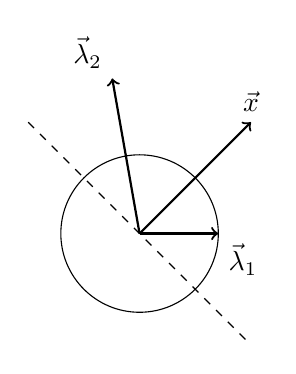
\begin{tikzpicture}
    %\fill[gray!50,opacity=0.7] (0,0) circle (\radius); 
    %\fill[gray!10, opacity=1] (0,0) -- (135:\radius) arc (135:315:\radius) -- cycle; 
    \draw[] circle(\radius);
    \draw[thick,->] (0,0,0) -- (\radius,0,0) node[anchor=north west]{$\vec{\lambda}_1$};
    \draw[thick,->] (0,0,0) -- (-0.3473, 1.9696,0) node[anchor=south east]{$\vec{\lambda}_2$};
    \draw[thick,->] (0,0,0) -- (1.4142, 1.4142,0) node[anchor=south]{$\vec{x}$};
    \draw[dashed] (-1.414,1.414,0) -- (1.414,-1.414,0) node[anchor=south]{};    
\end{tikzpicture}

%\tdplotsetmaincoords{40}{0}
%\tdplotsetrotatedcoords{150}{50}{20}
%\begin{tikzpicture}[scale=2,line join=bevel,tdplot_rotated_coords,fill %opacity=1,declare function={ colorFunc(\t)=ifthenelse(\t>0,60,300);}]
%\pgfsetlinewidth{.0pt}
%    \tdplotsphericalsurfaceplot[parametricfill]{72}{36}{2}%{transparent!0}{colorFunc(180*floor(\tdplotphi/180))
%    }{}{}{}
%\end{tikzpicture}

\subsubsection{Bell with two qubits}
The entanglement scenario is a straight-forward adaptation of the previously discussed prepare-and-measure scenario on any entangled qudit-qubit state. In this case, Alice chooses a random local POVM on a $d_Q$-dimensional quantum system, and produces an output according to the marginal distribution of her POVM elements. Based on her output, she computes Bob's entangled qubit post-measurement state, which is sent to Bob using the classical protocol for the prepare-and-measure scenario. Given that Bob's post-measurement qubit state is communicated by Alice using the existing prepare-and-measure classical protocol, the classical cost of the qubit transmission will be exactly the same.

\subsubsection{Bell with singlet state}
In a Bell scenario, there is a bipartite quantum system of two entangled and separated qubits, one with Alice and another one with Bob. The global state of the system is the entangled Bell singlet state $\ket{\psi^{-}}=\frac{1}{\sqrt{2}}(\ket{01} - \ket{10})$. Alice and Bob measure their own qubits along different basis and, while both outcomes appear random, their joint probabilities are correlated.

The entanglement scenario is a straight-forward adaptation of the previously discussed prepare-and-measure scenario on any entangled qudit-qubit state. In this case, Alice chooses a random local POVM on a $d_Q$-dimensional quantum system, and produces an output according to the marginal distribution of her POVM elements. Based on her output, she computes Bob's entangled qubit post-measurement state, which is sent to Bob using the classical protocol for the prepare-and-measure scenario. Given that Bob's post-measurement qubit state is communicated by Alice using the existing prepare-and-measure classical protocol, the classical cost of the qubit transmission will be exactly the same.

Similarly to the prepare-and-measure scenario described in section \ref{section:pm}, it is not possible to reproduce the correlations using a classical protocol with shared random variables without allowing classical communication among Alice and Bob once they have selected their measurements \cite{bell1964}. 
